\documentclass[10pt,a4paper, margin=1in]{article}
\usepackage{fullpage}
\usepackage{amsfonts, amsmath, pifont}
\usepackage{amsthm}
\usepackage{graphicx}
\usepackage{tikz}
\usepackage[utf8]{inputenc}
\usepackage{float}
\usepackage{pgfplots} 
\pgfplotsset{compat=newest} 
\usepackage{tkz-euclide}

\usepackage{geometry}
 \geometry{
 a4paper,
 total={210mm,297mm},
 left=10mm,
 right=10mm,
 top=10mm,
 bottom=10mm,
 }
 \begin{filecontents}{q3.dat}
 w   X(jw) 
 2   2  
 -2   2
\end{filecontents}
 % Write both of your names here. Fill exxxxxxx with your ceng mail address.
 \author{
  KOŞAR, Sinan Talha\\
  \texttt{e2099190@ceng.metu.edu.tr}
  \and
  DOĞAN, Furkan\\
  \texttt{e2098937@ceng.metu.edu.tr}
}
\title{CENG 384 - Signals and Systems for Computer Engineers \\
Spring 2018-2019 \\
Written Assignment 4}
\begin{document}
\maketitle



\noindent\rule{19cm}{1.2pt}

\begin{enumerate}

\item 
    \begin{enumerate}
    % Write your solutions in the following items.
    \item %write the solution of q1a
    $y[n] - \dfrac{3}{4}y[n-1] + \dfrac{1}{8}y[n-2] = 2x[n]$
    \item %write the solution of q1b
    We know that $x[n] = e^{jwn}$ and $y[n] = H(e^{jw}) e^{jwn}$, by placing to the equation found in part a of question 1:\\
    
    $H(e^{jw}) e^{jwn} - \dfrac{3}{4}H(e^{jw}) e^{jw(n-1)} + \dfrac{1}{8}H(e^{jw}) e^{jw(n-2)} = 2 e^{jwn}$\\
    
    $H(e^{jw}) e^{jwn} (1 - \dfrac{3}{4} e^{-jw} + \dfrac{1}{8}e^{-2jw}) = 2 e^{jwn}$\\
    
    $H(e^{jw}) = \dfrac{16}{e^{-2jw} -6 e^{-jw} + 8}$\\
    
    $=\dfrac{8}{-4 + e^{-jw}} - \dfrac{8}{-2 + e^{-jw}}$\\
    
    \item %write the solution of q1c
    We know $H(e^{jw}) = \sum_n h[n] e^{-jwn}$, we assume that 
    
    $h[n] = 0 for n < 0$, which is causal.\\
    We can shape the equation by using Fourier Transform of:\\
    
    $x[n] = a^n u[n] \xrightarrow{\text{FT}} \dfrac{1}{1-a e^{-jw}}$\\
    
    $H(e^{jw}) = \dfrac{-2}{1 - \dfrac{1}{4} e^{-jw}} + \dfrac{4}{1 - \dfrac{1}{2} e^{-jw}} \xrightarrow{\text{FT}} h[n] = (-2)(\dfrac{1}{4})^n u[n] + 4 (\dfrac{1}{2})^n u[n]$\\
    
    \item %write the solution of q1d
    $x[n] = (\dfrac{1}{4})^n u[n] \xrightarrow{\text{FT}} \dfrac{1}{1-\dfrac{1}{4} e^{-jw}} = X(e^{jw})$\\
    
    $Y(e^{jw}) = H(e^{jw}) X(e^{jw})$\\
    
    $=(\dfrac{8}{-4 + e^{-jw}} - \dfrac{8}{-2 + e^{-jw}})(\dfrac{4}{4-e^{-jw}})$\\
    
    $\dfrac{32}{(4-e^{-jw})(e^{-jw}-4)} -  \dfrac{32}{(4-e^{-jw})(e^{-jw}-2)}$\\
    
    $=(\dfrac{32}{4-e^{-jw}})(\dfrac{1}{e^{-jw}-4} -\dfrac{1}{e^{-jw}-2})$\\
    
    $=\dfrac{8}{1-\dfrac{1}{4}e^{-jw}}(\dfrac{\dfrac{-1}{4}}{1-\dfrac{1}{4}e^{-jw}}-\dfrac{\dfrac{-1}{2}}{1-\dfrac{1}{2}e^{-jw}})$\\
    
    By using same Fourier Transform,\\
    
    $8(\dfrac{1}{4})^n u[n](\dfrac{-1}{4}(\dfrac{1}{4})^n u[n] + \dfrac{1}{2}(\dfrac{1}{2})^n u[n]) = y[n]$
    \end{enumerate}


\item %write the solution of q2
$h_1 [n] \xrightarrow{\text{FT}} H_1 (e^{jw}) = \dfrac{1}{1-\dfrac{1}{3}e^{-jw}} = \dfrac{3}{3-e^{-jw}}$\\
since,\\
$\sum_{k=0}^{\infty} \alpha^k = \dfrac{1}{1-\alpha}$, so $x[n] = a^{n} u[n] \xrightarrow{\text{FT}} X(e^{jw}) = \dfrac{1}{1-a e^{-jw}}$\\
Let $x=e^{-jw}$\\
$H(z) = H_1(z) + H_2(z)$\\
$H_2 (z) = \dfrac{5z-12}{z^2 -7z + 12} - \dfrac{3}{3-z} = \dfrac{5z-12+3(z-4)}{(z-4)(z-3)} = \dfrac{8}{z-4}$\\
$=-2 \dfrac{1}{1-\dfrac{1}{4}z} \xrightarrow{} h_2(n)=-2(\dfrac{1}{4})^n u[n]$
\item      
    \begin{enumerate}
    \item %write the solution of q3a
    $sinc(\alpha t) \xrightarrow{\text{FT}} \dfrac{1}{\sqrt{2\pi \alpha^2}} . rect(\dfrac{w}{2\pi \alpha})$\\
    $\dfrac{sin 2 \pi t}{\pi t} \xrightarrow{\text{FT}} X_1 (w) = \dfrac{2}{\sqrt{2 \pi^3}} rect(\dfrac{w}{2 \pi^3})$\\
    $cos 3 \pi t \xrightarrow{\text{FT}} X_2 (w) = \pi [\delta(w+3\pi)+\delta(w-3\pi)]$\\
    $X(w) = \dfrac{2}{\sqrt{2\pi^3}} rect(\dfrac{w}{2\pi^3}) + \pi[\delta(w+3\pi)+\delta(w-3\pi)]$\\
   \begin{figure} [h!]
    \centering
    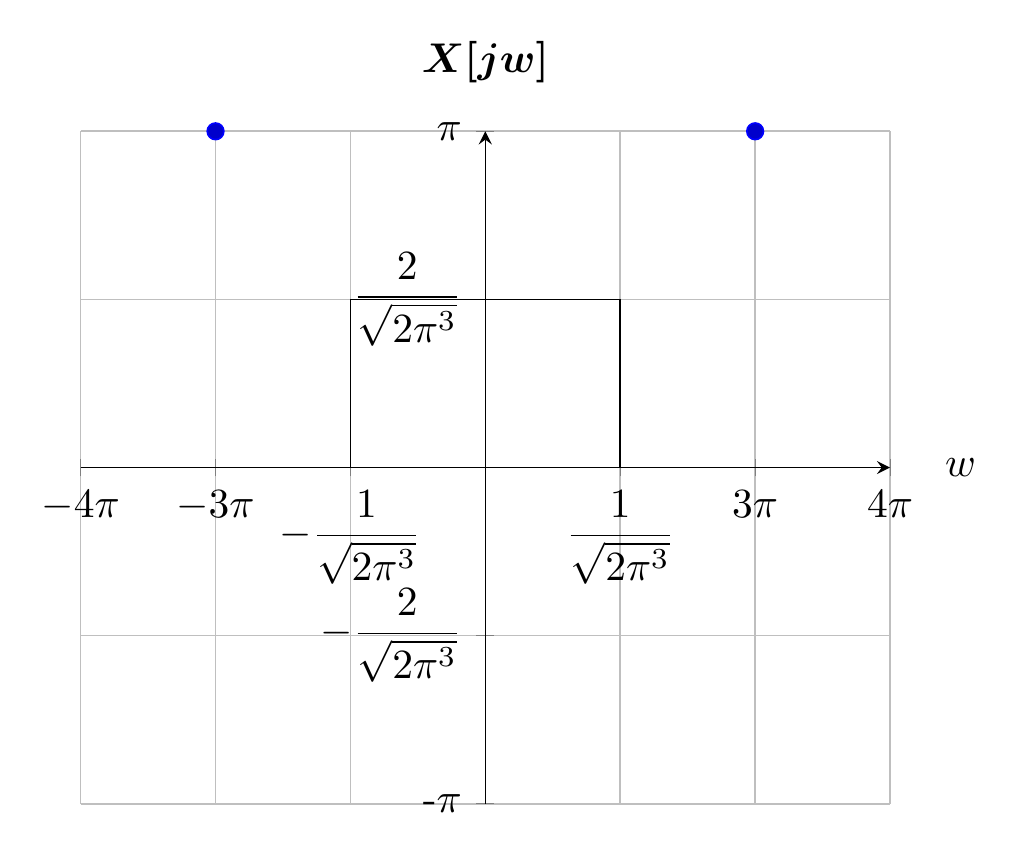
\begin{tikzpicture}[scale=1.5] 
      \begin{axis}[
          axis lines=middle,
          xlabel={$w$},
          ylabel={$\boldsymbol{X[jw]}$},
          xtick={ -3,-2,-1, 0,1,2, 3},
          xticklabels={$-4\pi$,$-3\pi$,$-\dfrac{1}{\sqrt{2\pi^3}}$,0,$\dfrac{1}{\sqrt{2\pi^3}}$,$3\pi$,$4\pi$},
          ytick={-2,-1, 0, 1,2},
          yticklabels={-$\pi$,$-\dfrac{2}{\sqrt{2\pi^3}}$,0,$\dfrac{2}{\sqrt{2\pi^3}}$,$\pi$},
          ymin=-2, ymax=2,
          xmin=-3, xmax=3,
          every axis x label/.style={at={(ticklabel* cs:1.05)}, anchor=west,},
          every axis y label/.style={at={(ticklabel* cs:1.05)}, anchor=south,},
          grid,
        ]
         \draw (-1,0) rectangle (1,1);
        \addplot+[only marks] coordinates {(2,2) (-2,2)};
      \end{axis}
    \end{tikzpicture}
    \caption{$w$ vs. $X[jw]$.}
    \label{fig:q3}
\end{figure}
       \item %write the solution of q3b
        The frequency for each term is a follows:\\
        Term1 $w_1 = 2\pi$\\
        Term2 $w_2 = 3\pi$\\
        Maximum Signal Frequency  $w_m = 3\pi$\\
        Sampling theorem says that $w_s > 2w_m = 6\pi$\\
        Therefore Nyquist frequency is $6\pi$\\
        Nyquist period $= \dfrac{2\pi}{ws} = \dfrac{1}{3}$
       \item %write the solution of q3c
       We know that:\\
       $X_p(jw) = \dfrac{1}{T_s}\sum_{k=-\infty}^{\infty} X_c(j(w-kw_s))$\\
       Put the findings to the equation\\
       $X_p(jw) = \dfrac{1}{\dfrac{1}{3}} \sum_{k=-\infty}^{\infty} Xc(j(w-k6\pi))$\\
      $X_p(jw) = 3 \sum_{k=-\infty}^{\infty} \dfrac{2}{\sqrt{2\pi^3}} rect(\dfrac{w-k6\pi}{2\pi^3}) + \pi[\delta(w-k6\pi+3\pi)+\delta(w-k6\pi-3\pi)]$
      \begin{figure} [H]
    \centering
    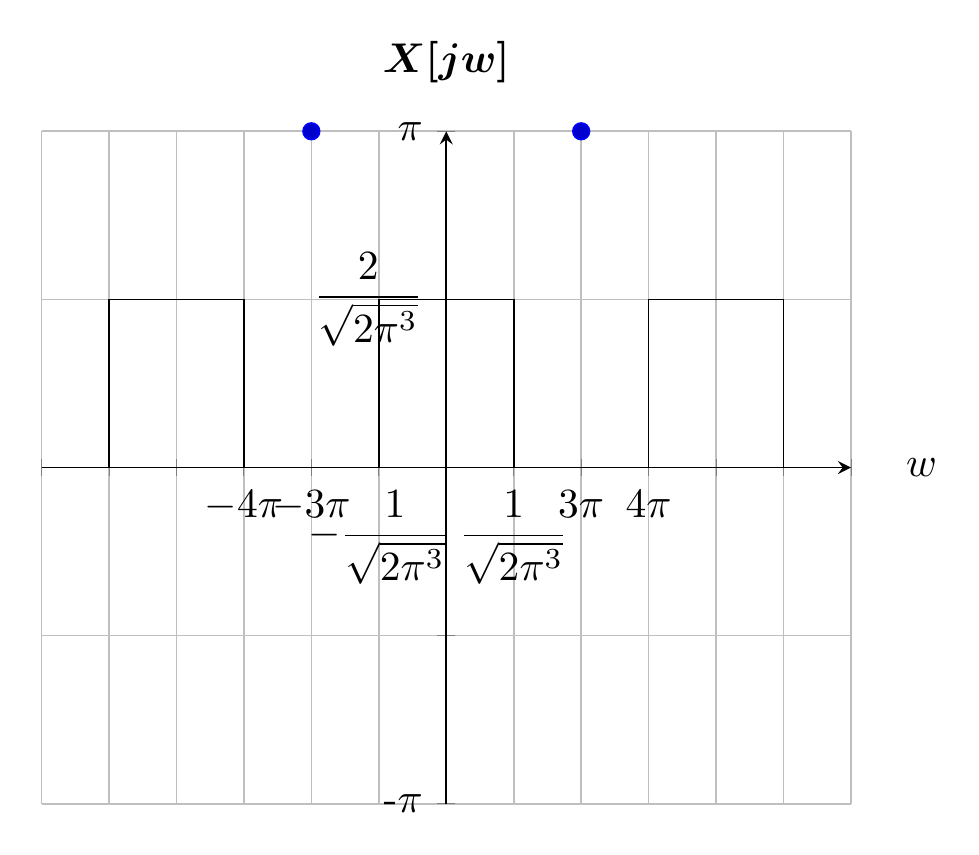
\begin{tikzpicture}[scale=1.5] 
      \begin{axis}[
          axis lines=middle,
          xlabel={$w$},
          ylabel={$\boldsymbol{X[jw]}$},
          xtick={ -6,-5,-4,-3,-2,-1, 0,1,2, 3,4,5,6},
          xticklabels={,,,$-4\pi$,$-3\pi$,$-\dfrac{1}{\sqrt{2\pi^3}}$,0,$\dfrac{1}{\sqrt{2\pi^3}}$,$3\pi$,$4\pi$,,,},
          ytick={-2,-1, 0, 1,2},
          yticklabels={-$\pi$,,0,$\dfrac{2}{\sqrt{2\pi^3}}$,$\pi$},
          ymin=-2, ymax=2,
          xmin=-6, xmax=6,
          every axis x label/.style={at={(ticklabel* cs:1.05)}, anchor=west,},
          every axis y label/.style={at={(ticklabel* cs:1.05)}, anchor=south,},
          grid,
        ]
         \draw (-1,0) rectangle (1,1);
          \draw (3,0) rectangle (5,1);
           \draw (-3,0) rectangle (-5,1);
        \addplot+[only marks] coordinates {(2,2) (-2,2)};
      \end{axis}
    \end{tikzpicture}
    \caption{$w$ vs. $X[jw]$.}
    \label{fig:q3}
\end{figure}
    \end{enumerate}

\item 
    \begin{enumerate}
    \item %write the solution of q4a
    $w=\pi$, so $T=\dfrac{2\pi}{w} = 2$\\
    We know the formulas for $X_p$:\\
    
    1)$X_p(jw) = \dfrac{1}{T}\sum_{k=-\infty}^{\infty} X(j(w-kw_s))$\\
    
    2)$X_d(e^{jw}) = X_p(j\dfrac{w}{T})$\\
    
$X_d(jw) = \dfrac{1}{2}\sum_{k=-\infty}^{\infty} X(j(\dfrac{w}{2}-k\pi)) = \dfrac{1}{2}\sum_{k=-\infty}^{\infty} \dfrac{2w}{\pi}-4k =\sum_{k=-\infty}^{\infty} \dfrac{w}{\pi}-2k$\\

for $|\dfrac{w}{2}-\pi k| \leq \dfrac{\pi}{4}, 0$ otherwise.
    \item %write the solution of q4b
    $h[n] \xrightarrow{\text{FT}} H(e^{jw})$\\
    
     As in question 3 part a:\\
     
     $cos \pi t \xrightarrow{\text{FT}} H(e^{jw})=\pi \sum_{k=-\infty}^{\infty}{\delta(w+ \pi -2\pi k)+\delta(w+\pi -2\pi k)}$
    \item %write the solution of q4c
    We know the multiplication property for fourier series:\\
    $y[n] \xrightarrow{\text{FT}} Y_d(e^{jw}) = \dfrac{1}{2\pi} X_d(e^{jw})*H(e^{jw})$\\
    
    We can take $X_d and H$ from part a and b\\
    
    $Y_d(e^{jw}) = \pi \sum_{k=-\infty}^{\infty} ((\sum_{l=-\infty}^{\infty} \dfrac{k}{\pi}-2l) \sum_{m=-\infty}^{\infty}{\delta(w-k+ \pi -2\pi m)+\delta(w-k+\pi -2\pi m)})$\\
    
    for $|\dfrac{w}{2}-\pi k| \leq \dfrac{\pi}{4}, 0$ otherwise.
    \end{enumerate}



\end{enumerate}
\end{document}

